\documentclass[xcolor=pdftex,dvipsnames,table,mathserif,aspectratio=169]{beamer}
\usetheme{metropolis}

\usepackage[english]{babel}
\usepackage{pgf,pgfarrows,pgfnodes,pgfautomata,pgfheaps}
\usepackage{amsmath,amssymb,setspace,centernot}
\usepackage[latin1]{inputenc}
\usepackage[T1]{fontenc}
\usepackage{relsize}
\usepackage{pdfpages}
\usepackage[absolute,overlay]{textpos} 

\newenvironment{reference}[2]{% 
  \begin{textblock*}{\textwidth}(#1,#2) 
      \footnotesize\it\bgroup\color{red!50!black}}{\egroup\end{textblock*}} 

\DeclareMathSizes{10}{10}{6}{6} 
\AtBeginSection[]{
  \begin{frame}
  \vfill
  \centering
  \begin{beamercolorbox}[sep=8pt,center,shadow=true,rounded=true]{title}
    \usebeamerfont{title}\insertsectionhead\par%
  \end{beamercolorbox}
  \vfill
  \end{frame}
}


\DeclareMathOperator*{\argmax}{arg\,max}
\DeclareMathOperator*{\argmin}{arg\,min}

\newcommand{\norm}[1]{\left\lVert#1\right\rVert}
\newcommand{\X}{\mathtt{X}}
\newcommand{\Y}{\mathtt{Y}}

%\newcommand{\R}{\mathbb{R}}
%\newcommand{\E}{\mathbb{E}}
%\newcommand{\V}{\mathbb{V}}
\newcommand{\p}{\mathbb{P}}
\newcommand*\df{\mathop{}\!\mathrm{d}}
\newcommand{\del}{\partial}

\begin{document}
\title{Supply and Instruments}
\author{Chris Conlon}
\institute{Grad IO}
\date{\today}

\frame{\titlepage}

\section{Adding Supply}
\begin{frame}{Supply}
\begin{itemize}
\item Economic theory gives us some additional powerful restrictions.
\item We may want to impose $MR = MC$.
\item Alternatively, we can ask -- what is a good instrument for demand? \alert{something from another equation} (ie: supply).
\end{itemize}
\end{frame}

\begin{frame}{Some setup}
We can break up the parameter space into three parts:
\begin{itemize}
\item $\theta_1$: linear exogenous demand parameters, 
 \item $\theta_2$: parameters including price and random coefficients (endogenous / nonlinear)
 \begin{itemize}
 \item $\theta_2 = [\alpha, \widetilde{\theta}_2]$
\end{itemize}
 \item $\theta_3$: linear exogenous supply parameters.
\end{itemize}
\end{frame}



\begin{frame}[plain]
\frametitle{Supply Side}
Consider the multi-product Bertrand FOCs:
\footnotesize
{\begin{eqnarray*}
\arg \max_{p \in \mathcal{J}_f} \pi_f (\mathbf{p}) &=& \sum_{j \in \mathcal{J}_f} (p_j - c_j) \cdot s_j(\mathbf{p}) +  \kappa_{fg}\sum_{k \in \mathcal{J}_g} (p_k - c_k) \cdot s_k(\mathbf{p}) \\
0&=& s_j(\mathbf{p}) + \sum_{k \in \mathcal{J}_f} (p_k - c_k) \frac{\partial s_{k}}{\partial p_j}(\mathbf{p}) 
\end{eqnarray*}
}
It is helpful to define the \alert{ownership matrix} $\Omega_{(j,k)}(\mathbf{p})  = - \frac{\partial s_{j}}{\partial p_k}(\mathbf{p})$:
\begin{eqnarray*}
A(\kappa)_{(j,k)} = \left\{\begin{array}{lr}
          1 & \text{for }  (j,k) \in \mathcal{J}_f \text{ for any } f \\ 
	  0 & \text{o.w}\\
        \end{array} \right\}
\end{eqnarray*}
We can re-write the FOC in matrix form where $\odot$ denotes Hadamard product (element-wise):
\begin{eqnarray*}
        s(\mathbf{p}) &= (A \odot \Omega(\mathbf{p})) \cdot (\mathbf{p} - \mathbf{mc}), \\
       \mathbf{mc} &=  \mathbf{p} - \underbrace{(A \odot \Omega(\mathbf{p}))^{-1} s(\mathbf{p})}_{\eta(\mathbf{p},\mathbf{s},\theta_2)}.
\end{eqnarray*}
\end{frame}



\begin{frame}{Recovering Marginal Costs }
Recover implied markups/ marginal costs, and assume a functional form for $mc_{jt}(x_{jt},w_{jt})$.
\begin{eqnarray*}
\widehat{\mathbf{mc}}(\theta_2)&=& \mathbf{p}- \Omega(\mathbf{p},\theta_2)^{-1} q(\mathbf{p},\theta_2)\\
f(mc_{jt}) &=& h_s(x_{jt} , w_{jt},\theta_3)+ \omega_{jt}
\end{eqnarray*}
Which we can solve for $\omega_{jt}$:
\begin{eqnarray*}
\omega_{jt} &=&  f(\mathbf{p}- \Omega(\mathbf{p},\theta_2)^{-1} q(\mathbf{p},\theta_2)) - h_s(x_{jt},w_{jt},\theta_3)
\end{eqnarray*}
\begin{itemize}
\item $f(\cdot)$ is usually $\log(\cdot)$ or identity.
\item $h_s(x_{jt},w_{jt},\theta_3) = [x_{jt}, \, w_{jt}] \gamma$ is usually linear
\item I can use this to form additional moments: $E[\omega_{jt}' Z_{jt}^{s}]=0$.
%\item I can just stack these up with the demand moments $E[\xi_{jt}' Z_{jt}^d]=0$.
%\item Now I have $\dim(Z^d) + \dim(Z^s)$ moments altogether.
\i%tem This step is optional but can aid in identification (if you believe it).
\end{itemize}
\end{frame}



\begin{frame}{Simultaneous Supply and Demand}
\tiny
\begin{enumerate}[(a)]
\item For each market $t$: solve $\mathcal{S}_{jt} = s_{jt}(\delta_{\cdot t},\theta_2)$ for $\widehat{\delta}_{\cdot t}(\theta_2)$.
\item For each market $t$: use $\widehat{\delta}_{\cdot t}(\theta_2)$ to construct $\eta_{\cdot 
t}(\mathbf{q_t},\mathbf{p_t},\widehat{\delta}_{\cdot t}(\theta_2),\theta_2)$
\item For each market $t$: Recover $\widehat{mc}_{jt}(\widehat{\delta}_{\cdot t}(\theta_2),\theta_2) = p_{jt} - \eta_{jt}(\widehat{\delta}_{\cdot t}(\theta_2),\theta_2)$
\item Stack up $\widehat{\delta}_{\cdot t}(\theta_2)$ and $\widehat{mc}_{jt}(\widehat{\delta}_{\cdot t}(\theta_2),\theta_2)$ and use linear IV-GMM to recover $[\widehat{\theta}_1(\theta_2), \widehat{\theta}_3(\theta_2) ]$ following the recipe in Appendix
\item Construct the residuals:
\begin{align*}
\nonumber    \widehat{\xi}_{jt}(\theta_2) &= \widehat{\delta}_{jt}(\theta_2) -  x_{jt} \widehat{\beta}(\theta_2) + \alpha p_{jt}\\
    \widehat{\omega}_{jt}(\theta_2) &= \widehat{mc}_{jt}(\theta_2) -  [x_{jt}\, w_{jt}]\, \widehat{\gamma}(\theta_2)
\end{align*}
\item Construct sample moments
\begin{align*}
\nonumber g_n^D(\theta_2)=\frac{1}{N} \sum_{jt} Z_{jt}^{D\prime} \widehat{\xi}_{jt}(\theta_2)\\
 g_n^S(\theta_2)=\frac{1}{N} \sum_{jt} Z_{jt}^{S \prime} \widehat{\omega}_{jt}(\theta_2)
\end{align*}
\item Construct GMM objective $Q_n(\theta_2)= \left[ {\begin{array}{c} g_n^d(\theta_2) \\ g_n^s(\theta_2) \end{array} } \right]' W  \left[ {\begin{array}{c} g_n^d(\theta_2) \\ g_n^s(\theta_2) \end{array} } \right] $
\end{enumerate}
\end{frame}

\begin{frame}{Additional Details}
Some different definitions:
\begin{alignat}{3}
\label{eq:stacked}
\nonumber y_{jt}^D &:= \widehat \delta_{jt}(\theta_2) + \alpha p_{jt} &=(x_{jt} \-\ v_{jt})' \beta + \xi_t &=: x_{jt}^{D\prime}\beta + \xi_{jt} \\ 
y_{jt}^S &:= \widehat{mc}_{jt}(\theta_2) &= (x_{jt} \-\ w_{jt})'\gamma + \omega_t &=: x_{jt}^{S\prime} \gamma + \omega_{jt} 
\end{alignat}
Stacking the system across observations yields:\footnote{Note: we cannot perform independent regressions unless we are willing to assume that $Cov(\xi_{jt},\omega_{jt})=0$.}
\begin{align}
\underbrace{\begin{bmatrix} y_D \\ y_S \end{bmatrix}}_{2N\times1} = 
\underbrace{\begin{bmatrix}
X_D & 0 \\
0 & X_S 
\end{bmatrix}}_{2N\times(K_1+K_3)}
\underbrace{\begin{bmatrix}
\beta \\ \gamma %\Gamma_D \\ \Gamma_S
\end{bmatrix}}_{(K_1+K_3)\times1} + 
\underbrace{\begin{bmatrix}
\xi \\ \omega % \varepsilon_D \\ \varepsilon_S
\end{bmatrix}}_{2N\times 1}
\end{align}
\end{frame}

%
%
%
%\begin{frame}{Supply Side as Instruments }
%\begin{itemize}
%\item Instruments for demand depend on \alert{exclusion restrictions}
%\item Where do instruments come from? Something omitted that appears in another equation.
%\end{itemize}
%\begin{eqnarray*}
%p_{jt}  &=& c_{jt}(w_{jt},x_{jt}) +  \frac{s_{jt}(\mathbf{p_t})}{\left|\frac{\partial s_{jt}(\mathbf{p_t})}{\partial p_{jt}}\right|}  +\sum_{k \in \mathcal{J}_f} (p_k - c_k) \frac{\frac{ \partial s_{kt}}{\partial p_{jt}}(\mathbf{p_t})}{\left|\frac{\partial s_{jt}(\mathbf{p_t})}{\partial p_{jt}}\right|}  
%\end{eqnarray*}
%\begin{enumerate}
%\item Exogenous regressors $x_{jt}$.
%\item Cost shifters: $w_{jt}$ (hard to find in practice), Hausman instruments.
%\item Markup shifters:  $ \frac{s_{jt}(\mathbf{p_t})}{\frac{\partial s_{jt}(\mathbf{p_t})}{\partial p_{jt}}}$ \\(function of $(p_j,x_j,\xi_j, p_{-j},x_{-j},\xi_{-j})$).
%\end{enumerate}
%\end{frame}
%

\section{Instruments and Identification}
\begin{frame}{Parametric Identifcation}
\begin{itemize}
\item Once we have $\delta_{jt}(\theta)$ identification of linear parameters is pretty straightforward
\begin{eqnarray*}
\delta_{jt}(\theta) = x_{jt} \beta - \alpha p_{jt} + \xi_j + \xi_t + \Delta \xi_{jt}
\end{eqnarray*}
\item This is either basic linear IV or panel linear IV.
\item How are $\sigma$ taste parameters identified?
\begin{itemize}
\item Consider increasing the price of $j$ and measuring substitution to other products $k,k'$ etc.
\item If sales of $k$ increase with $p_j$ and $(x_j^{(1)},x_k^{(1)})$ are similar then we increase the $\sigma$ that corresponds to $x^{(1)}$.
\item Price is the most obvious to vary, but sometimes this works for other characteristics (like distance).
\item Alternative: vary the set of products available to consumers by adding or removing an option.
\end{itemize}
\end{itemize}
\end{frame}




\begin{frame}{Instruments}
\begin{itemize}
\item Recall the nested logit, where there are two separate endogeneity problems
\begin{itemize}
\item \alert{Price}: this is the familiar one!
\item \alert{Nonlinear characteristics} $\sigma$ this is the other one.
\end{itemize}
\item We are doing nonlinear GMM: Start with $E[\xi_{jt} | x_{jt}, z_{jt}]=0$ use $E[\xi' [Z X]]=0$.
\begin{itemize}
\item In practice this means that for valid instruments $(x,z)$ any function $f(x,z)$ is also a valid instrument $E[ \xi_{jt} f(x_{jt},z_{jt})]=0$.
\item We can use $x, x^2, x^3,\ldots$ or interactions $x \cdot z, x^2 \cdot z^2, \ldots$.
\item What is a reasonable choice of $f(\cdot)$?
\item Where does $z$ come from?
\end{itemize}
\end{itemize}
\end{frame}


\begin{frame}{Exclusion Restrictions}
\begin{eqnarray*}
    \delta_{jt}(\mathcal{S}_t,\widetilde{\theta}_2) &=&  [x_{jt}, \alert{v_{jt}}]  \beta  - \alpha p_{jt} + \xi_{jt}\\
    f(p_{jt} - \eta_{jt}(\theta_2,\mathbf{p},\mathbf{s})) &=&   h(x_{jt},\alert{w_{jt}};\theta_3)+\omega_{jt}
\end{eqnarray*}
The first place to look for exclusion restrictions/instruments:
\begin{itemize}
\item Something in another equation!
\item $v_j$ shifts demand but not supply
\item $w_j$ shifts supply but not demand
\item If it doesn't shift either is it really relevant?
\end{itemize}
\end{frame}


\begin{frame}{Markup Shifters}
The equilibrium markup is a function of \alert{everything!} $\eta_{jt}(\mathbf{p},\mathbf{s},\xi_t,\omega_t,x_{t},w_{t},v_t,\theta_2)$:
\begin{itemize}
\item It is literally \alert{endogenous} (depends on error terms)!
\item But lots of potential instruments beyond \alert{excluded} $v_t$ or $w_t$.
\item Also $v_{-j}$ and $w_{-j}$ and $x_{-j}$.
\item Not $p_{-j}$ or $\xi_{-j}$, etc.
\item The idea is that these instruments shift the \alert{marginal revenue curve}.
\item What is a good choice of $f(x_{-j})$? etc.
\end{itemize}
\end{frame}




\begin{frame}{BLP Instruments}
\begin{itemize}
\item Common choices are average characteristics of other products in the same market $f(x_{-j,t})$. \alert{BLP instruments}
\begin{itemize}
\item Same firm $z_{1jt} = \overline{x}_{-j_f,t} = \frac{1}{\left\vert{F_j}\right\vert}  \sum_{k \in \mathcal{F}_j} x_{kt} - \frac{1}{\left\vert{F_j}\right\vert} x_{jt}$.
\item Other firms $z_{2jt}=\overline{x}_{\cdot t} - \overline{x}_{-j_f,t} - \frac{1}{J} x_{jt}$.
\item Plus regressors $(1, x_{jt})$.
\item Plus higher order interactions 
\end{itemize}
\item Technically linearly independent for large (finite) $J$, but becoming highly correlated.
\begin{itemize}
\item Can still exploit variation in number of products per market or number of products per firm.
\end{itemize}
\item Correlated moments $\rightarrow$ ``many instruments''.
\begin{itemize}
\item May be inclined to ``fix'' correlation in instrument matrix directly.
\end{itemize}
\end{itemize}
\end{frame}


\begin{frame}{Armstrong (2016): Weak Instruments?}
Consider the limit as $J \rightarrow \infty$
\begin{eqnarray*}
\frac{s_{jt}(\mathbf{p_t})}{\left|\frac{\partial s_{jt}(\mathbf{p_t})}{\partial p_{jt}}\right|} = \frac{1}{\alpha} \frac{1}{1-s_{jt}} \rightarrow \frac{1}{\alpha}
\end{eqnarray*}
\begin{itemize}
\item Hard to use markup shifting instruments to instrument for a constant.
\item How close to the constant do we get in practice?
\item Average of $x_{-j}$ seems like an especially poor choice. Why?
\item Shows there may still be some power in: products per market, products per firm.
\item Convergence to constant extends to mixed logits (see Gabaix and Laibson 2004).
\item Suggests that you really need cost shifters.
\end{itemize}
\end{frame}

\begin{frame}{Differentiation Instruments: Gandhi Houde (2017)}
\begin{itemize}
\item Also need instruments for the $\Sigma$ or $\sigma$ random coefficient parameters.
\item Instead of average of other characteristics $f(x) = \frac{1}{J-1} \sum_{k \neq j} x_k$, can transform as distance to $x_j$.
\begin{eqnarray*}
d_{jt} ^k=  x_k - x_j  
\end{eqnarray*}
\item And use this transformed to construct two kinds of IV (Squared distance, and count of local competitors)
\begin{eqnarray*}
DIV_1 =& \sum_{j \in F}  d_{jt}^2,  \quad &\sum_{j \notin F}  d_{jt}^2 \\
DIV_2 =& \sum_{j \in F}  I[d_{jt} < c]   \quad &\sum_{j \notin F}   I[d_{jt} < c]
\end{eqnarray*}
\item They choose $c$ to correspond to one standard deviation of $x$ across markets.
\end{itemize}
\end{frame}


\begin{frame}{Optimal Instruments}
\begin{itemize}
\item Since any $f(x,z)$ satisfies our orthogonality condition, we can try to choose $f(x,z)$ as a \alert{basis} to approximate optimal instruments.
\item This is challenging in practice -- and in fact suffers from a curse of dimensionality.
\item This is frequently given as a rationale behind higher order $x$'s.
\item When the dimension of $x$ is low -- this may still be feasible. ($K \leq 3)$.
\end{itemize}
\end{frame}


\begin{frame}{Optimal Instruments}
\noindent Chamberlain (1987) tells us the optimal instruments for this supply-demand system of $G\Omega^{-1}$ where for a given observation $n$, 

\begin{align*}
G_n &:= \underbrace{\begin{bmatrix}
\frac{\del \xi}{\del \beta} & \frac{\del \omega}{\del \beta} \\
\frac{\del \xi}{\del \alpha} & \frac{\del \omega}{\del \alpha} \\
\frac{\del \xi}{\del \sigma} & \frac{\del \omega}{\del \sigma} \\
\frac{\del \xi}{\del \gamma} & \frac{\del \omega}{\del \gamma} 
\end{bmatrix}_n}_{(K_1 + K_2 + K_3)\times 2}
= \begin{bmatrix}
-x & 0 \\
\xi_\alpha & \omega_\alpha \\
\xi_\sigma & \omega_\sigma \\
0 & -x \\
0 & -w
\end{bmatrix}_n 
\quad  
\Omega := \underbrace{\begin{bmatrix}
v_\xi^2 & v_{\xi \omega} \\
v_{\xi \omega} & v_\omega^2
\end{bmatrix}}_{2 \times 2}
\end{align*}
\end{frame}


\begin{frame}{\#4: Optimal Instruments}
\begin{align*}
G_n\Omega^{-1} = \frac{1}{v_\xi^2 v_\omega^2 - (v_{\xi \omega})^2}\times \begin{bmatrix}
-v_\omega^2 x & \alert{v_{\xi \omega}x} \\
v_\omega^2 \xi_\alpha - v_{\xi \omega}\omega_\alpha & v_\xi^2 \omega_\alpha - v_{\xi \omega}\xi_\alpha \\
v_\omega^2 \xi_\sigma - v_{\xi \omega}\omega_\sigma & v_\xi^2 \omega_\sigma - v_{\xi \omega}\xi_\sigma \\
\alert{v_{\xi \omega}x }&  -v_\xi^2 x \\
v_{\xi \omega}w & -v_\xi^2 w
\end{bmatrix}_n
\end{align*}
\noindent Clearly rows 1 and 4 are co-linear. 
\end{frame}

\begin{frame}{\#4: Optimal Instruments}
\begin{align*}
(G_n\Omega^{-1} )\circ \Theta= \frac{1}{v_\xi^2 v_\omega^2 - (v_{\xi \omega})^2}\times \begin{bmatrix}
-v_\omega^2 x & 0 \\
v_\omega^2 \xi_\alpha - v_{\xi \omega}\omega_\alpha & v_\xi^2 \omega_\alpha - v_{\xi \omega}\xi_\alpha \\
v_\omega^2 \xi_\sigma - v_{\xi \omega}\omega_\sigma & v_\xi^2 \omega_\sigma - v_{\xi \omega}\xi_\sigma \\
0 &  -v_\xi^2 x \\
v_{\xi \omega}w & -v_\xi^2 w
\end{bmatrix}_n
\end{align*}
\noindent Now we can partition our instrument set by column into ``demand'' and ``supply'' instruments as 
\begin{align*}
z_{nD} := (G_n\Omega^{-1} \circ \Theta)_{\cdot 1} \\
z_{nS} := (G_n\Omega^{-1} \circ \Theta )_{\cdot 2} 
\end{align*}
\end{frame}

\begin{frame}{Aside: What does Supply tell us about Demand?}
\begin{align*}
\del \alpha: v_\omega^2 \xi_\alpha - v_{\xi \omega}\omega_\alpha  \quad& v_\xi^2 \omega_\alpha - v_{\xi \omega}\xi_\alpha \\
\del \sigma: v_\omega^2 \xi_\sigma - v_{\xi \omega}\omega_\sigma \quad& v_\xi^2 \omega_\sigma - v_{\xi \omega}\xi_\sigma 
\end{align*}
\begin{itemize}
\item Under optimal IV these are \alert{overidentifying restrictions}
\item Maybe cases where one part of these instruments is trivial.
\end{itemize}
\end{frame}


\begin{frame}{Optimal Instruments}
How to construct optimal instruments in form of Chamberlain (1987)
\begin{eqnarray*}
E\left[\frac{\partial \xi_{jt}}{\partial \theta} | X_t, w_{jt} \right] = \left[\beta, E\left[\frac{\partial \xi_{jt}}{\partial \alpha} | X_t, w_{jt} \right] , E\left[\frac{\partial \xi_{jt}}{\partial \sigma} | X_t, w_{jt} \right] \right]
\end{eqnarray*}
Some challenges:
\begin{enumerate}
\item $p_{jt}$ depends on $X_{t}, w_{t}, \xi_{t}$ in a highly nonlinear way (no explicit solution!).
\item $E[\frac{\partial \xi_{jt}}{\partial \sigma} | X_t, w_{t} ] =E[[\frac{\partial \mathbf{s_t}}{\partial \mathbf{\delta_t}}]^{-1} [\frac{\partial \mathbf{s_t}}{\partial \mathbf{\sigma}}] | X_t, w_{t} ]$  (not conditioned on endogenous $p$!)
\end{enumerate}
``Feasible'' Recipe:
\begin{enumerate}
\item Fix $\hat{\theta}=(\hat{\alpha},\hat{\beta},\hat{\sigma})$ and draw $\xi_t$ from empirical density
\item Solve fixed point equation for $\hat{p_{jt}}$
\item Compute necessary Jacobian
\item Average over all values of $\xi_t$. (Lazy approach: use only $\xi =0$).
\end{enumerate}
\end{frame}


\begin{frame}{Simplified Version: Reynaert Verboven (2014)}
\begin{itemize}
\footnotesize
\item Optimal instruments are easier to work out if $p = mc$.
\begin{eqnarray*}
c = p  + \underbrace{\Delta^{-1} s}_{\rightarrow 0}  = X \gamma_1 + W \gamma_2 + \omega
\end{eqnarray*}
\item Linear cost function means linear reduced-form price function.
\begin{eqnarray*}
E\left[ \frac{\partial \xi_{jt} }{\partial \alpha} | z_t \right] &=& E[p_{jt} | z_t] = x_{jt} \gamma_1 + w_{jt} \gamma_2\\
E\left[ \frac{\partial \omega_{jt} }{\partial \alpha} | z_t \right] &=& 0 , \quad E\left[ \frac{\partial \omega_{jt} }{\partial \sigma} | z_t \right] = 0\\
E\left[ \frac{\partial \xi_{jt} }{\partial \sigma} | z_t \right] &=&E\left[ \frac{\partial \delta_{jt} }{\partial \sigma} | z_t \right]\\
\end{eqnarray*}
\item If we are worried about endogenous oligopoly markups is this a reasonable idea?
\item Turns out that the important piece tends to be \alert{shape} of jacobian for $\sigma_x$.
\end{itemize}
\end{frame}

\begin{frame}{Optimal Instruments: Reynaert Verboven (2014)}
\begin{center}
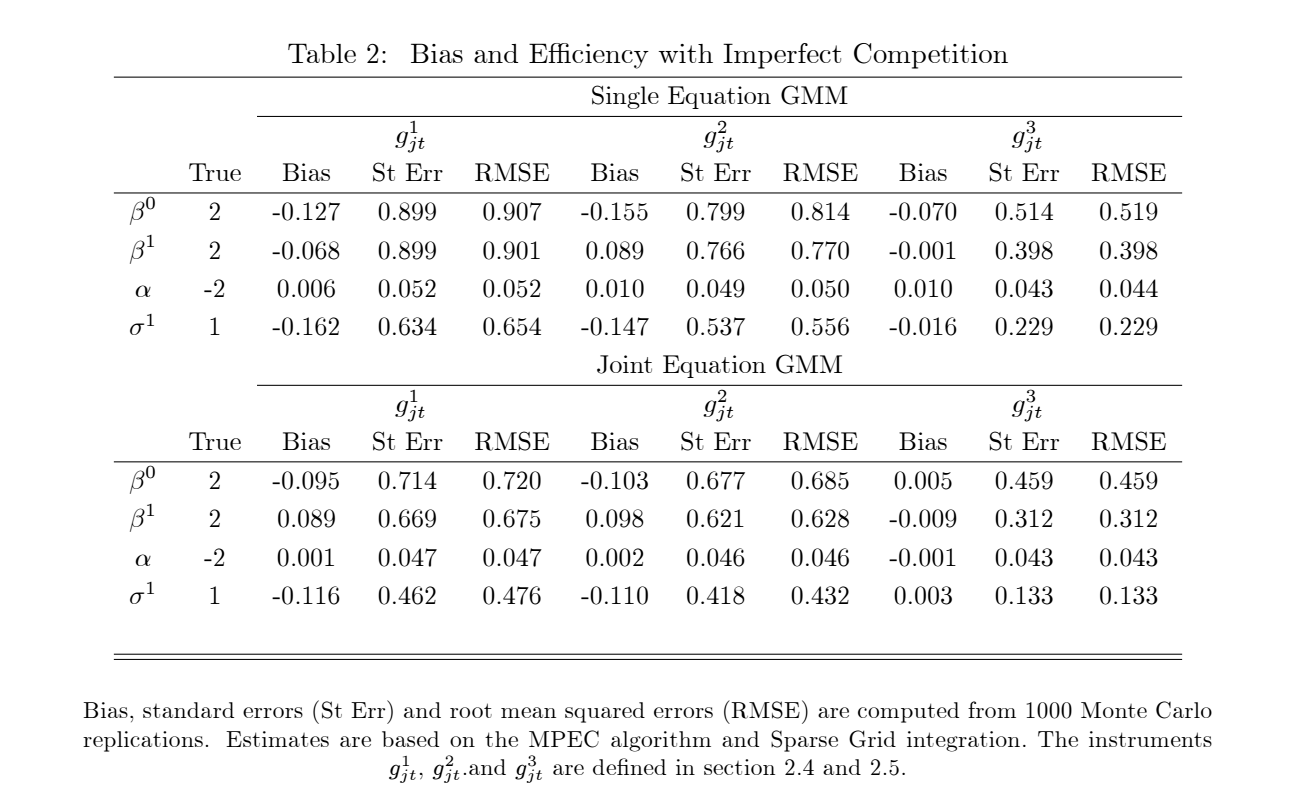
\includegraphics[width=4in]{resources/verboven.png}
\end{center}
\end{frame}


\begin{frame}{Differentiation Instruments: Gandhi Houde (2016)}
\begin{center}
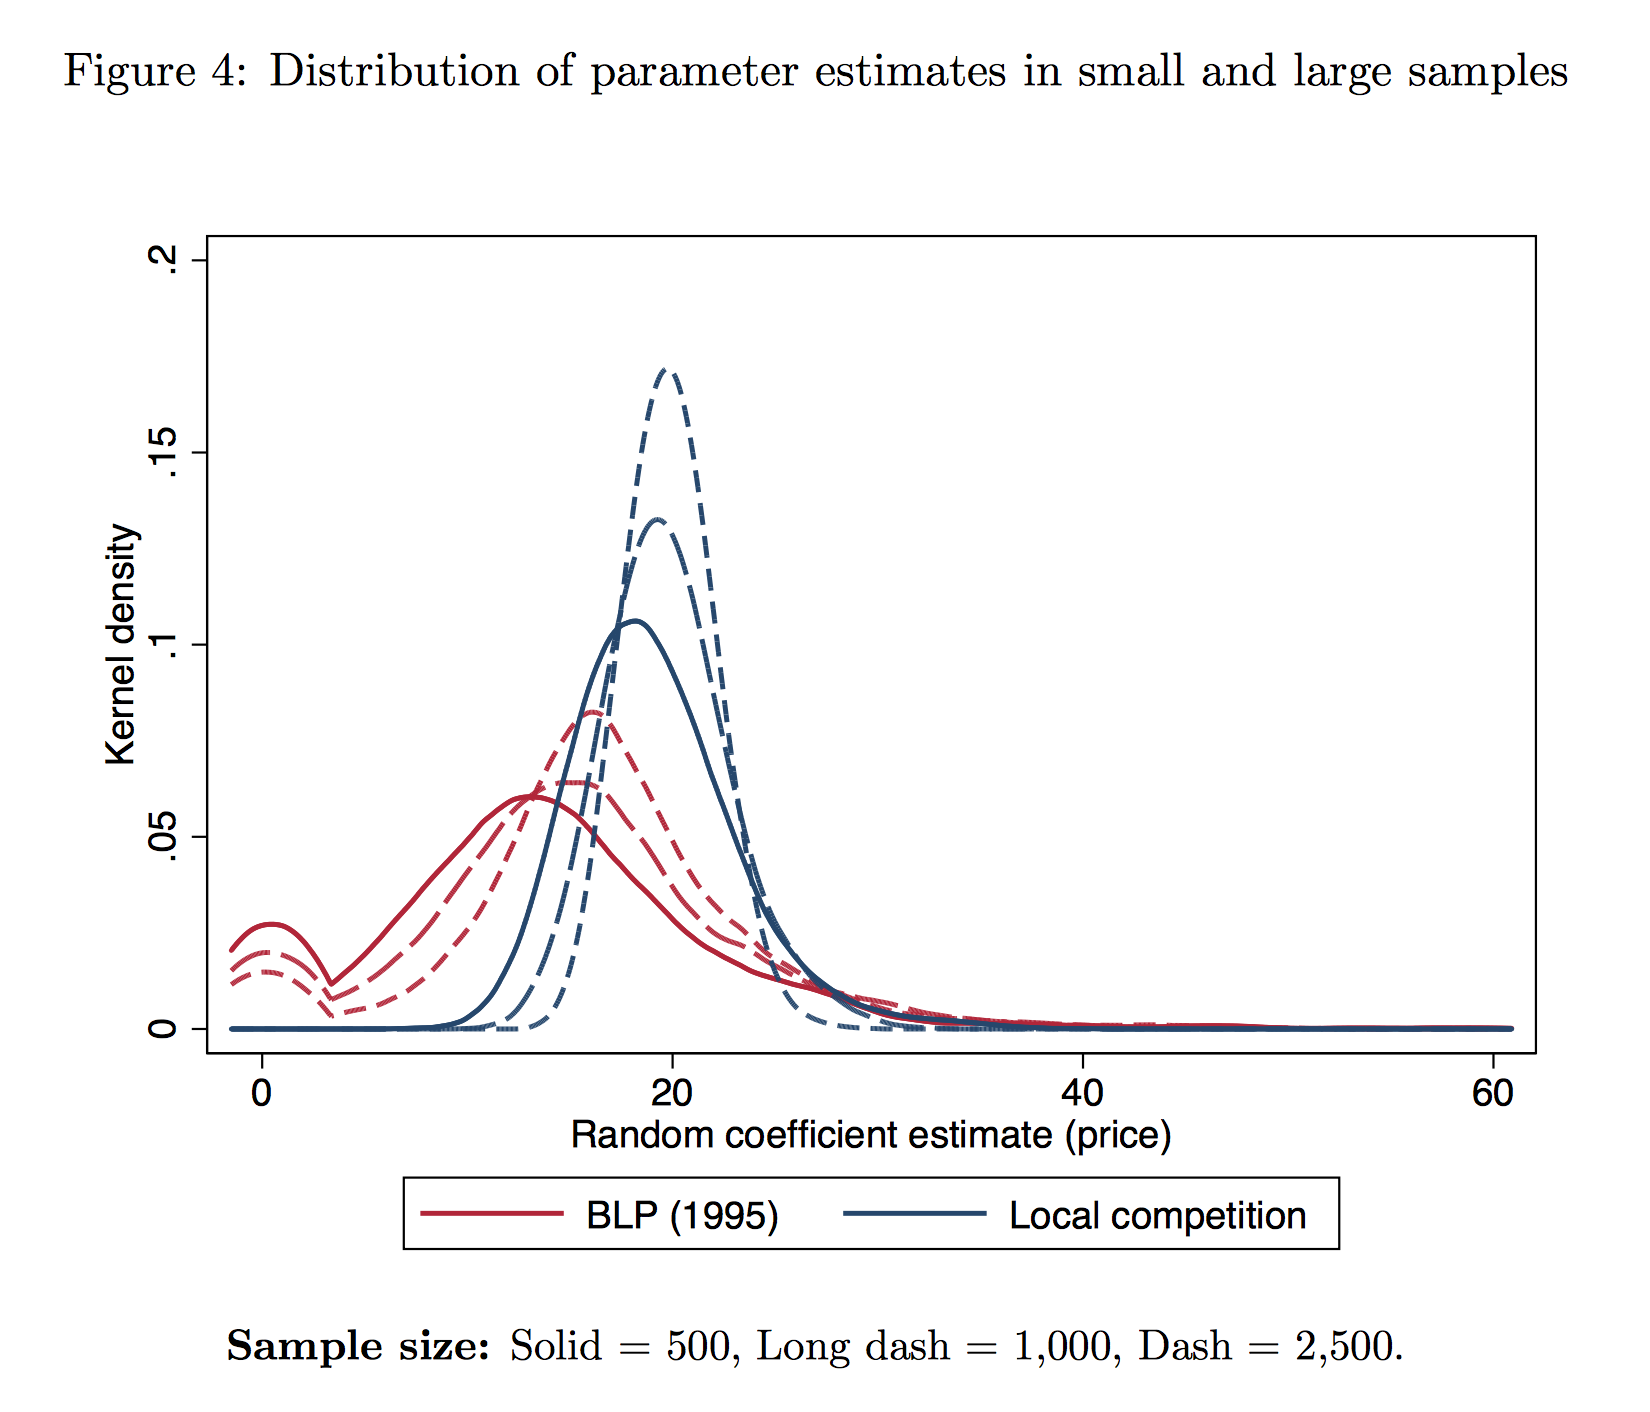
\includegraphics[width=3.8in]{resources/d_iv1.png}
\end{center}
\end{frame}


\begin{frame}{IV Comparison: Conlon and Gortmaker (2019)}
\begin{center}
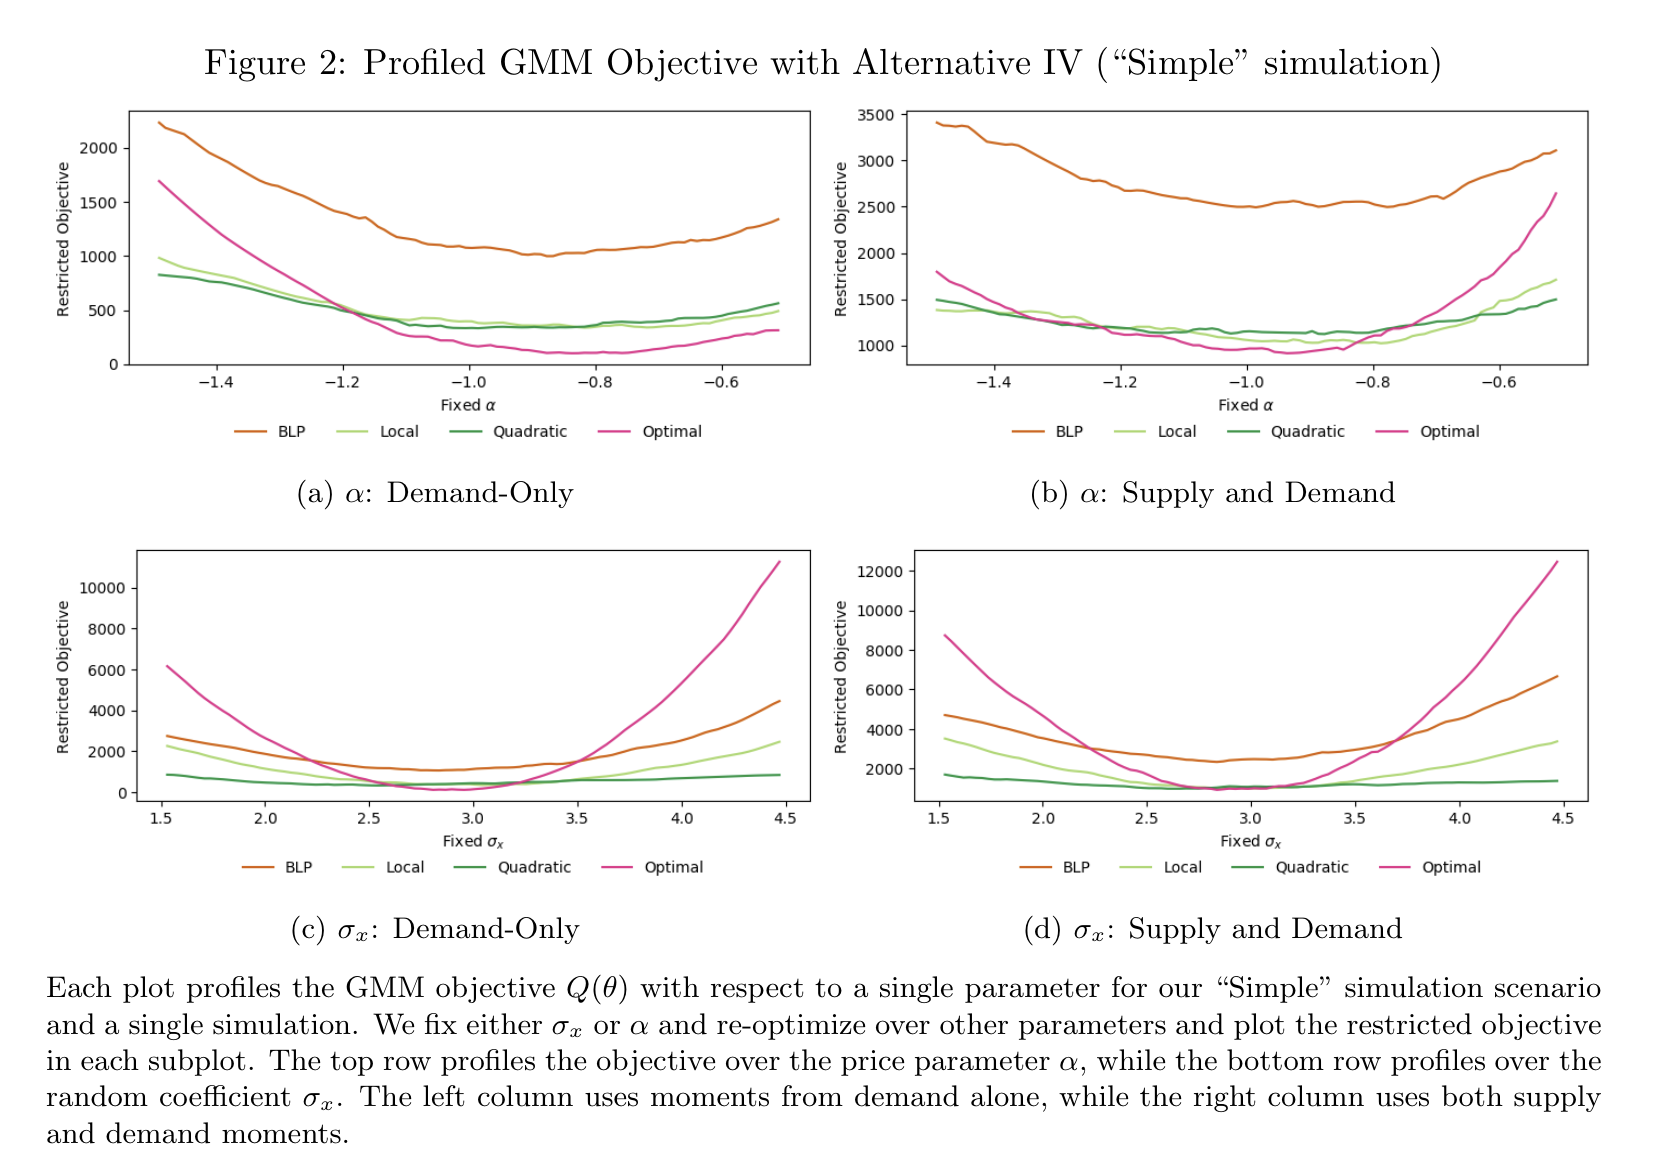
\includegraphics[width=3.9in]{resources/cg_figure.png}
\end{center}
\end{frame}




 \begin{frame}
\frametitle{BLP Alternatives}
\begin{itemize}
 \item BLP give us both a statistical \alert{estimator} and an \alert{algorithm} to obtain estimates.
\item Plenty of other algorithms exist
\begin{itemize}
\item We could solve for $\delta$ using the contraction mapping, using \texttt{fsolve} / Newton's Method / Guess and Check (not a good idea!).
\item We could try and consider a non-nested estimator for the BLP problem instead of solving for $\delta(\theta),\xi(\theta)$ we could let $\delta,\xi,\alpha,\beta$ be free parameters.
 \end{itemize}
\item We could think about different statistical estimators such as $K$-step GMM, Continuously Updating GMM, etc.
 \end{itemize}
\end{frame}


 \begin{frame}\frametitle{Dube Fox Su (2012)}
\footnotesize
\begin{eqnarray}
\label{blpnfxp}
\nonumber \arg \min_{\theta_2} && \psi' \Omega^{-1} \psi \quad \mbox{ s.t. } \\
\nonumber \psi &=& \xi(\theta_2)' Z\\
\xi_{jt}(\theta) &=& \delta_{jt}(\theta_2) - x_{jt} \beta - \alpha p_{jt} \\
\nonumber \log(S_{jt})  &=& \log(s_{jt}(\delta,\theta_2))
\end{eqnarray}

\begin{eqnarray}
\label{blpmpec}
\nonumber \arg \min_{\theta_2,\alpha,\beta, \xi,\psi} && \psi' \Omega^{-1}  \psi \quad \mbox{ s.t. } \\
 \psi &=& \xi' Z\\
\nonumber \xi_{jt} &=& \delta_{jt} - x_{jt} \beta - \alpha p_{jt} \\
\nonumber \log(S_{jt})  &=& \log(s_{jt}(\theta_2, \delta))
\end{eqnarray}
\end{frame}

\begin{frame}
\frametitle{Comparing Approaches}
\begin{itemize}
\item The original BLP paper and the DFS paper define different \alert{algorithms} to produce the same statistical \alert{estimator}.
\begin{itemize}
\item The BLP algorithm is a \alert{nested fixed point} (NFP) algorithm. 
\item The DFS algorithm is a \alert{mathematical program with equilibrium constraints} (MPEC).
\item The unknown parameters satisfy the same set of first-order conditions. (Not only asymptotically, but in finite sample).
\item $\hat{\theta}_{NFP} \approx \hat{\theta}_{MPEC}$ but for numerical differences in the optimization routine.
\end{itemize}
\item Our choice of algorithm should mostly be about computational convenience.
\end{itemize}
\end{frame}

\begin{frame}
\frametitle{BLP: NFP Advantages/Disadvantages}
\begin{itemize}
\item Advantages
\begin{itemize}
\item Concentrate out all of the linear in utility parameters $(\xi,\delta,\beta)$ so that we only search over $\Sigma$. When $\dim(\Sigma)=K$ is small (few dimensions of unobserved heterogeneity) this is a big advantage. For $K \leq 3$ this is my preferred approach.
\item When $T$ (number of markets/periods) is large then you can exploit solving in parallel for $\delta$ market by market.
\end{itemize}
\item Disadvantages
\begin{itemize}
\item Small numerical errors in contraction can be amplified in the outer loop, $\rightarrow$ tolerance needs to be very tight.
\item Errors in numerical integration can also be amplified in the outer loop $\rightarrow$ must use a large number of draws/nodes.
\item Hardest part is working out the Jacobian via IFT.
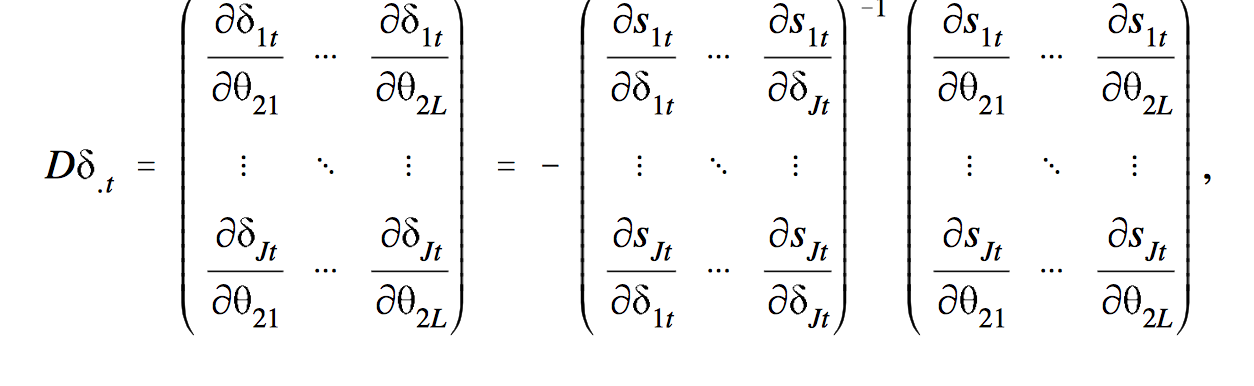
\includegraphics[width=2.8in]{resources/implicit_function.png}\\
\end{itemize}
\end{itemize}
\end{frame}

\begin{frame}
\frametitle{BLP: MPEC Advantages/Disadvantages}
\begin{itemize}
\item Advantages
\begin{itemize}
\item Problem scales better in $\dim(\Sigma)$.
\item Because all constraints hold at the optimum only: less impact of numerical error in tolerance or integration.
\item Derivatives are less complicated than $\frac{\partial \delta}{\partial \theta}$ (no IFT).
\end{itemize}
\item Disadvantages
\begin{itemize}
\item We are no longer concentrating out parameters, so there are a lot more of them! Storing the (Hessian) matrix of second derivatives can be difficult on memory.
\item We have to find the derivatives of the shares with respect to all of the parameters $\beta,\xi,\theta$. (The other derivatives are pretty easy).
\item Parallelizing the derivatives is trickier than NFP case.
\end{itemize}
\end{itemize}
\end{frame}


%
%\begin{frame}{Differentiation Instruments: Gandhi Houde (2016)}
%\begin{center}
%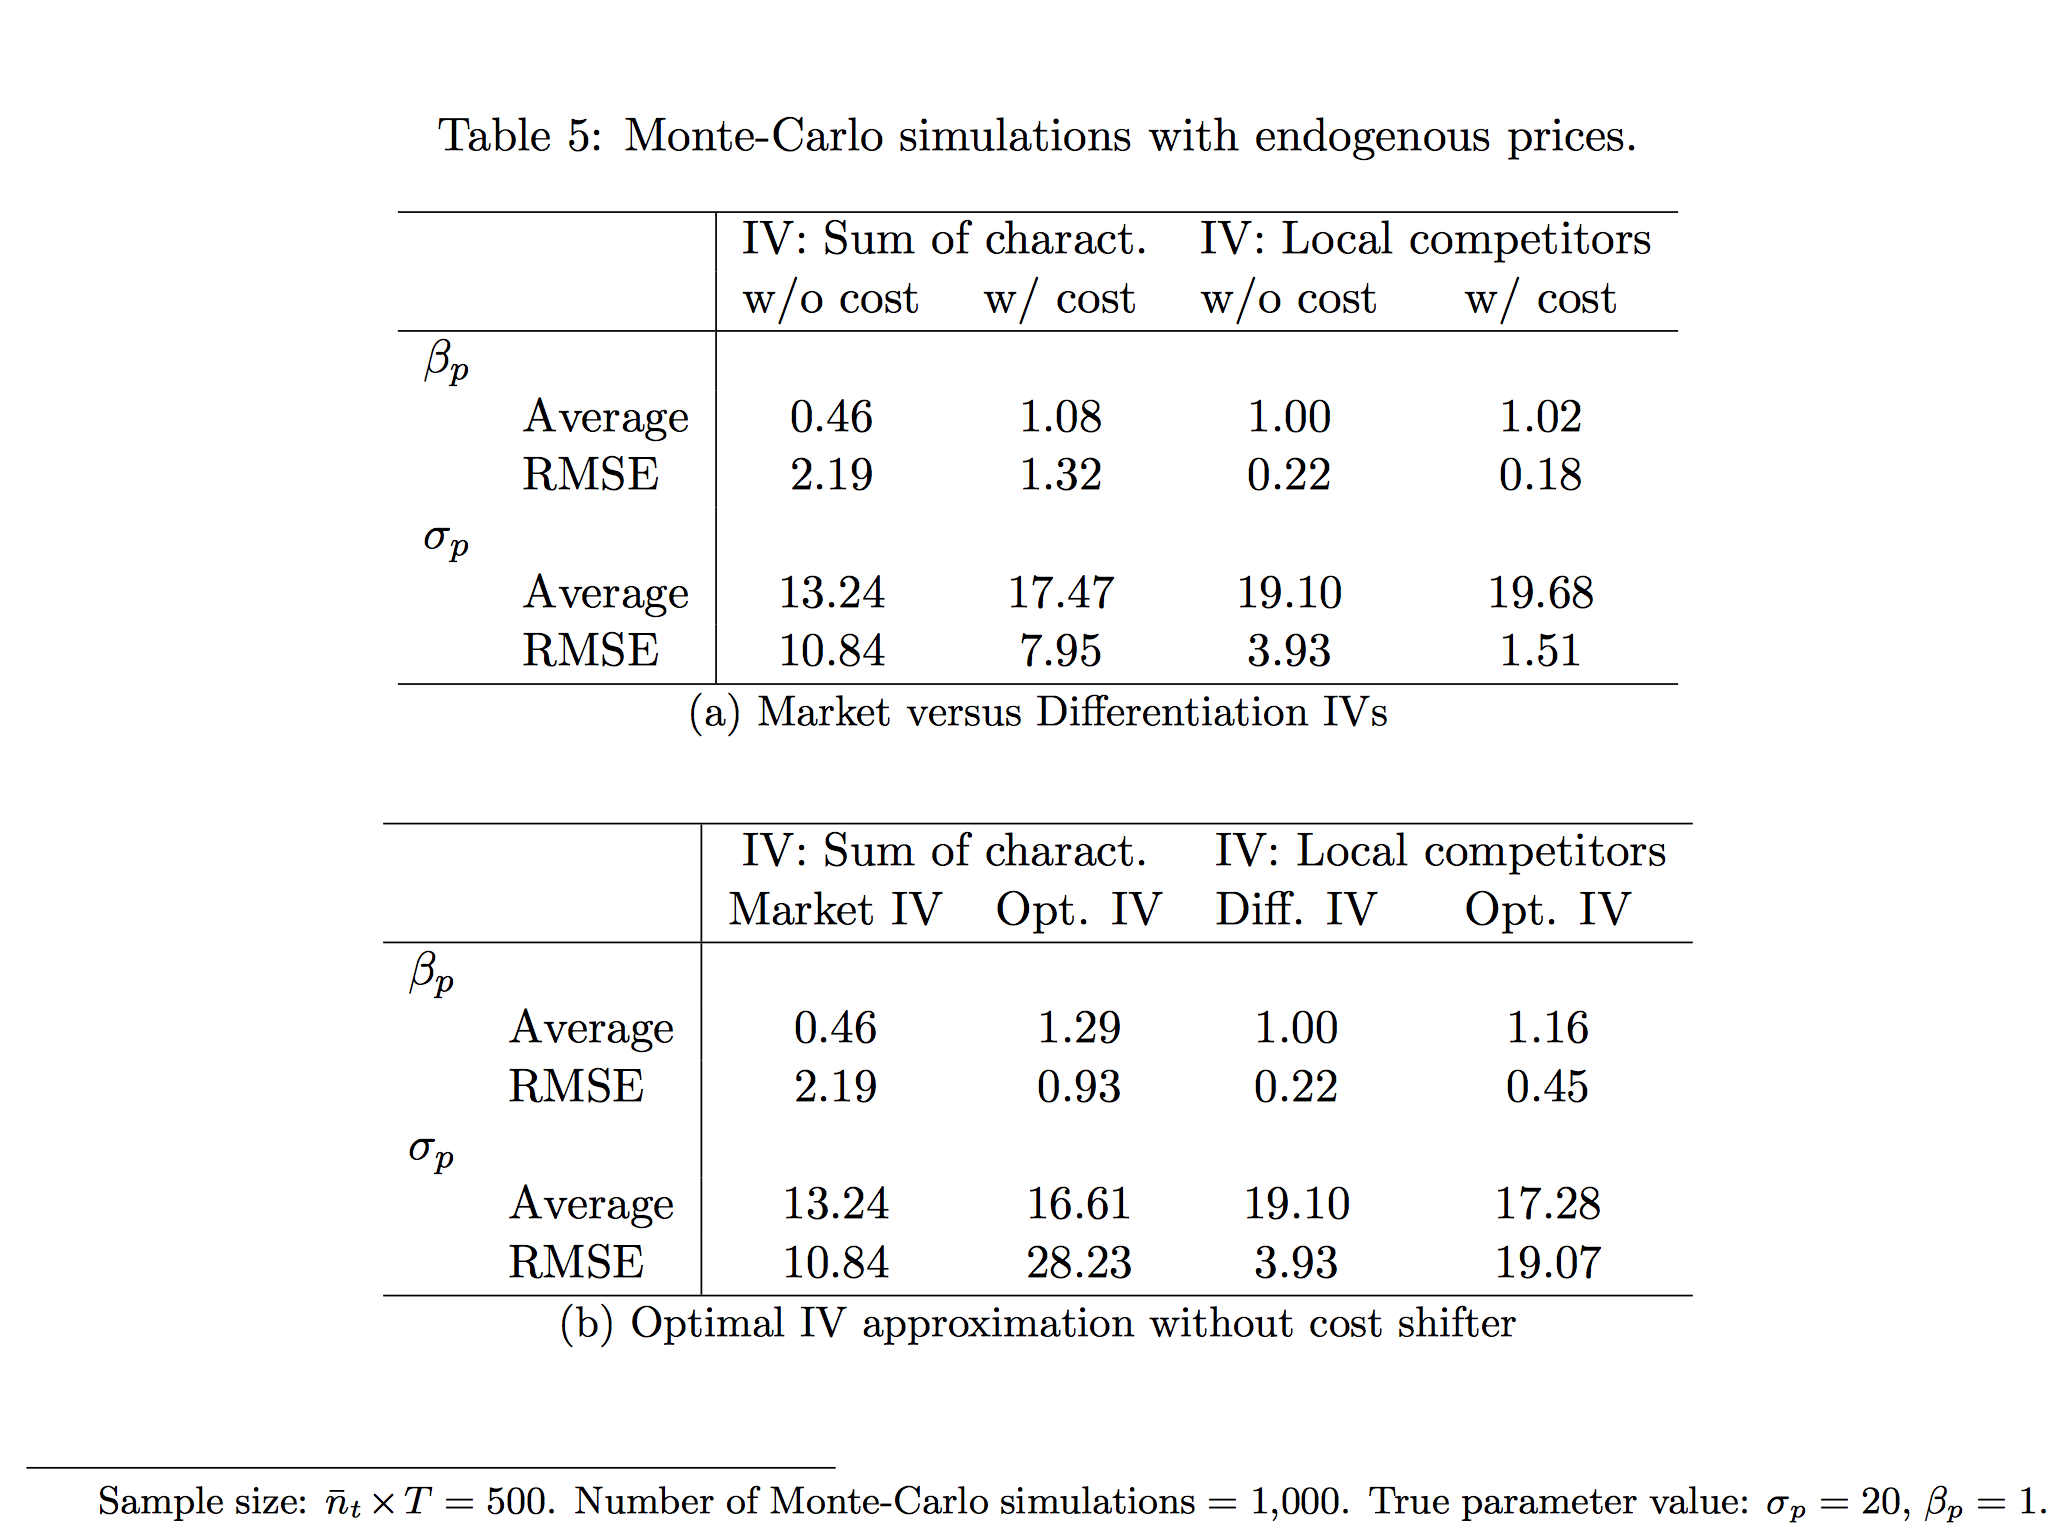
\includegraphics[width=3.8in]{resources/d_iv2.png}
%\end{center}
%\end{frame}
%



%
%\begin{frame} \frametitle{Extensions: Supply Moments}
%\begin{itemize}
%\item We can also impose the Bertrand FOC as a set of additional moments.
%\item First parametrize marginal cost
%\begin{eqnarray*}
%\ln mc_{jt} = \gamma_1 x_{jt} + \gamma_2 w_{jt} + \omega_{jt}
%\end{eqnarray*}
%\item helpful to constrain MC to be positive always.
%\item Note that for any vector of prices $p$ and demand parameters $\theta$ we can recover a unique vector of marginal costs (by solving the system of linear equations).
%\item Imposing the supply side only helps if we have information about the marginal costs / production function that we would like to impose
%\item Imposing these restrictions is helpful in constraining markups (so that implied MC are always positive, etc.).
%\item Misspecified functional forms for costs can cause problems!
%\end{itemize}
%\end{frame}





\end{document}